\tikzset{every picture/.style={line width=0.75pt}}
\begin{tikzpicture}
	\node[inner sep=0pt] (image1) {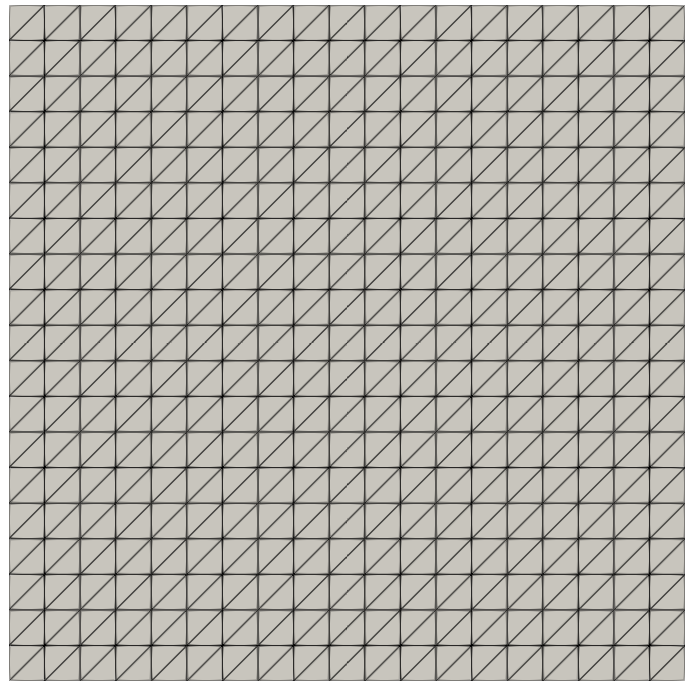
\includegraphics[width=0.25\linewidth]{chapter4/Figures/Stent/meshing_step_1.png}};
	\node[above right] at (image1.north west) {a) Initial Mesh};
	\node[inner sep=0pt,right=0.5cm of image1] (image2) {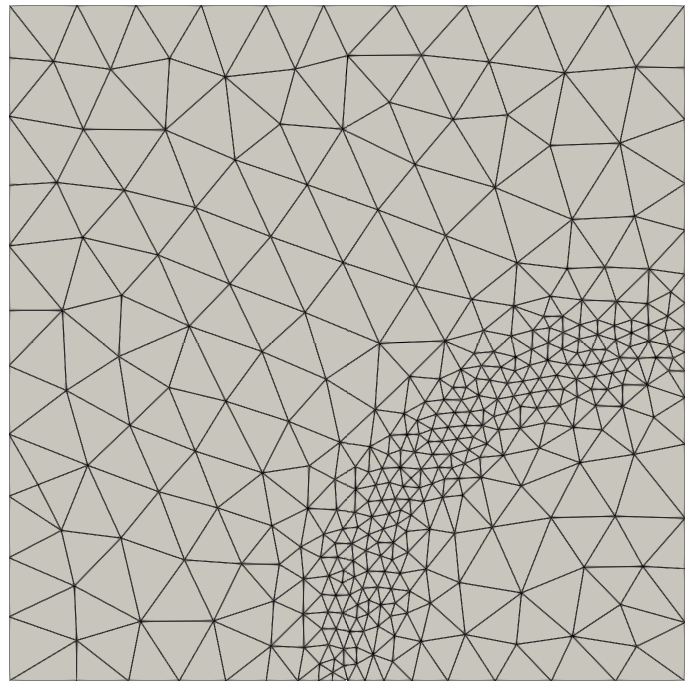
\includegraphics[width=0.25\linewidth]{chapter4/Figures/Stent/meshing_step_2.png}};
	\node[above right] at (image2.north west) {b) Interface refinement};
	\node[inner sep=0pt,below=0.9cm of image1] (image3) {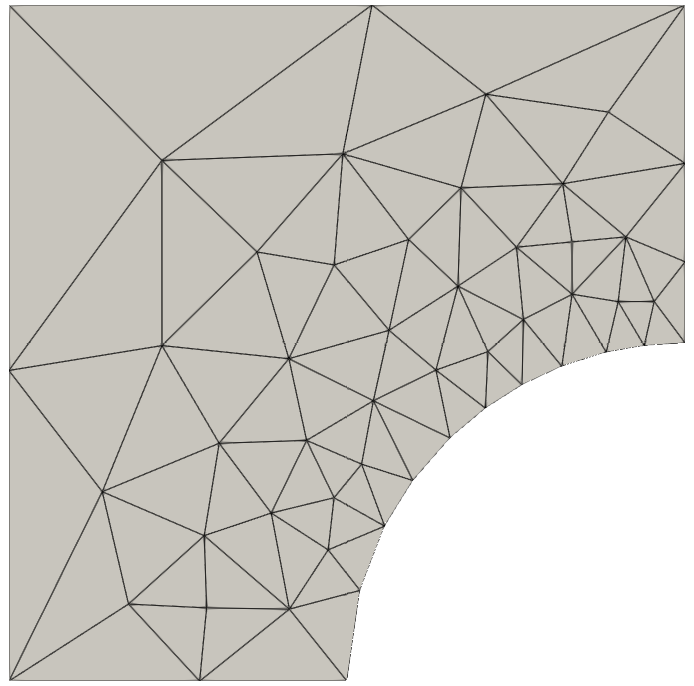
\includegraphics[width=0.25\linewidth]{chapter4/Figures/Stent/meshing_step_3.png}};
	\node[above right] at (image3.north west) {c) Isovalue splitting};
	\node[inner sep=0pt,right=0.5cm of image3] (image4) {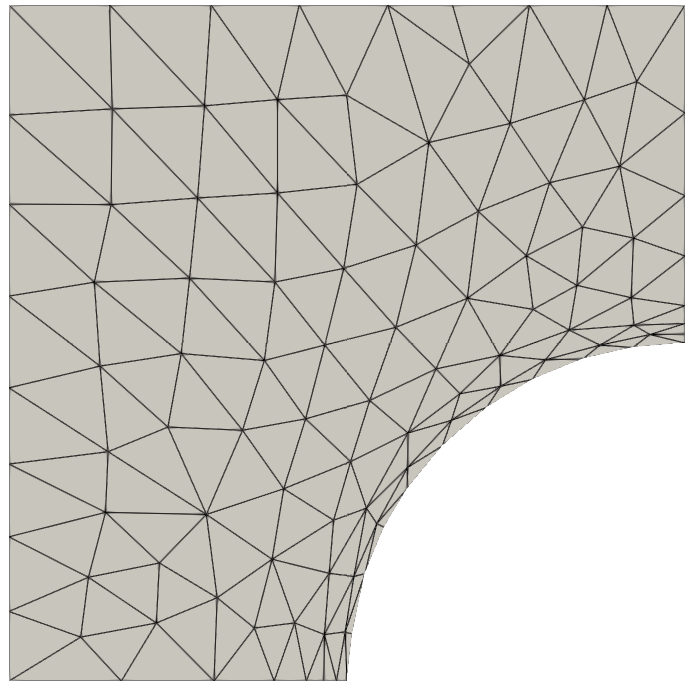
\includegraphics[width=0.25\linewidth]{chapter4/Figures/Stent/meshing_step_4.png}};
	\node[above right] at (image4.north west) {d) Boundary layers};
\end{tikzpicture}
